\documentclass[10pt]{article}  

%%%%%%%% PREÁMBULO %%%%%%%%%%%%
\title{Reporte de Laboratorio}
\usepackage{babel} %Indica que escribiermos en español
\usepackage[utf8]{inputenc} %Indica qué codificación se está usando ISO-8859-1(latin1)  o utf8  
\usepackage{amsmath} % Comandos extras para matemáticas (cajas para ecuaciones,
% etc)
\usepackage{amssymb} % Simbolos matematicos (por lo tanto)
\usepackage{longtable} %agregadom para hacer tablas
\usepackage{xltabular}
\usepackage{tabularray}
\usepackage{graphicx} % Incluir imágenes en LaTeX

\usepackage{color} % Para colorear texto
\definecolor{Blanco}{gray}{1}
\definecolor{Gray}{rgb}{0.501,0.501,0.501}
\definecolor{Tranquil}{rgb}{0.89,1,1}
\graphicspath{ {./images/} }

\usepackage{subfigure} % subfiguras
\usepackage{float} %Podemos usar el especificador [H] en las figuras para que se
% queden donde queramos
\usepackage{capt-of} % Permite usar etiquetas fuera de elementos flotantes
% (etiquetas de figuras)
\usepackage{sidecap} % Para poner el texto de las imágenes al lado
	\sidecaptionvpos{figure}{c} % Para que el texto se alinie al centro vertical
\usepackage{caption} % Para poder quitar numeracion de figuras
\usepackage{commath} % funcionalidades extras para diferenciales, integrales,
% etc (\od, \dif, etc)
\usepackage{cancel} % para cancelar expresiones (\cancelto{0}{x})
 
\usepackage{anysize} 					% Para personalizar el ancho de  los márgenes
\marginsize{2cm}{2cm}{2cm}{2cm} % Izquierda, derecha, arriba, abajo

\usepackage{appendix}
\renewcommand{\appendixname}{Apéndices}
\renewcommand{\appendixtocname}{Apéndices}
\renewcommand{\appendixpagename}{Apéndices} 
% Para que las referencias sean hipervínculos a las figuras o ecuaciones y
% aparezcan en color
\usepackage[colorlinks=true,plainpages=true,citecolor=blue,linkcolor=blue]{hyperref}
\usepackage{fancyhdr} 
\pagestyle{fancy}
\fancyhf{}
\fancyhead[L]{\footnotesize UNI} %encabezado izquierda
\fancyhead[R]{\footnotesize Fac. de Ciencias}   % dereecha
\fancyfoot[R]{\footnotesize Reporte}  % Pie derecha
\fancyfoot[C]{\thepage}  % centro
\fancyfoot[L]{\footnotesize Dinamica de Rotaci\'{o}n}  %izquierda
\renewcommand{\footrulewidth}{0.4pt}


\usepackage{listings} % Para usar código fuente
\definecolor{dkgreen}{rgb}{0,0.6,0} % Definimos colores para usar en el código
\definecolor{gray}{rgb}{0.5,0.5,0.5} 
% configuración para el lenguaje que queramos utilizar
\lstset{language=Matlab,
   keywords={break,case,catch,continue,else,elseif,end,for,function,
      global,if,otherwise,persistent,return,switch,try,while},
   basicstyle=\ttfamily,
   keywordstyle=\color{blue},
   commentstyle=\color{red},
   stringstyle=\color{dkgreen},
   numbers=left,
   numberstyle=\tiny\color{gray},
   stepnumber=1,
   numbersep=10pt,
   backgroundcolor=\color{white},
   tabsize=4,
   showspaces=false,
   showstringspaces=false}

\newcommand{\sen}{\operatorname{\sen}}	% Definimos el comando \sen para el seno
%en español

\title{Plantilla para Reportes IMEC-UTB}
% Basada en la plantilla para reportes UPIITA de  Overleaf

%%%%%%%% TERMINA PREÁMBULO %%%%%%%%%%%%

\begin{document}

%%%%%%%%%%%%%%%%%%%%%%%%%%%%%%%%%% PORTADA %%%%%%%%%%%%%%%%%%%%%%%%%%%%%%%%%%%%%%%%%%%%
																					%%%
\begin{center}																		%%%
\newcommand{\HRule}{\rule{\linewidth}{0.5mm}}									%%%\left
 																					%%%

\hspace{0.9cm}

\textsc{\huge Universidad Nacional de Ingeniería }\\[0.8cm]
			
\textsc{\LARGE Facultad de Ciencias}

\vspace{0.6cm}



\includegraphics[scale = 0.15]{UNI.png}

													 								%%%
\vspace*{0.6cm}								%%%
																					%%%	



\begin{minipage}{0.9\textwidth} 
\begin{center}																					%%%
\textsc{\LARGE  Laboratorio de Física CF1B2-B}
\end{center}
\end{minipage}\\[0.3cm]
%%%
    																				%%%
 			\vspace*{0.4cm}																		%%%
																					%%%
\HRule \\[0.5cm]																	%%%
{ \huge \bfseries Din\'{a}mica de Rotaci\'{o}n}\\[0.2cm]	%%%
 																					%%%
\HRule \\[0.9cm]																	%%%
 																				%%%
																					%%%
\begin{minipage}{0.46\textwidth}													%%%
\begin{flushleft} \large															%%%

% Aqui a continuación pongan los nombres de los integrantes
\emph{El grupo conformado por:}\\[2mm]
Vasquez Alvarado Luis Martin   \\20234143G \\[1mm]
Cortez Núñez Christian\\20232203B\\[1mm]
Rocca Cruz Axel\\20234046A\\[1mm]
 

%%%
			%\vspace*{2cm}	
            													%%%
										 						%%%
\end{flushleft}																		%%%
\end{minipage}		
																%%%
\begin{minipage}{0.52\textwidth}		
\vspace{-1.9cm}											%%%
\begin{flushright} \large															%%%
\emph{Profesor:}\\[2mm]																	%%%
AMORETTI VIDAL JESUS ESTEBAN \\ [1mm]NAUPA ROQUE ALEXANDER RAUL\\
\end{flushright}																	%%%
\end{minipage}	
\vspace*{1cm}
%\begin{flushleft}
 	
%\end{flushleft}
%%%																	%%%															
\vspace{-2.4cm}	
\begin{minipage}{0.98\textwidth}
\begin{flushright}	
        \textbf{Mesa : E7}
\end{flushright}
\end{minipage}

 \vspace{2.4cm}

\large{\today}\\
\vspace{0.3cm}

{ \Large\bfseries 2025-1}
										 			
\end{center}							 											
																					
\newpage																		
%%%%%%%%%%%%%%%%%%%% TERMINA PORTADA %%%%%%%%%%%%%%%%%%%%%%%%%%%%%%%%

\tableofcontents 
\newpage																		

\section{Introducción y objetivos del experimento}
Este informe se basa en datos obtenidos en el laboratorio de Física II de la Facultad de Ciencias. Se fundamenta en la guía de laboratorio y otras referencias citadas más adelante. Su objetivo es responder el cuestionario y comparar los resultados experimentales con la teoría. De acuerdo con la guía del laboratorio y las instrucciones del docente, el informe se organiza como sigue.

\subsection{Competencias generales}
\begin{itemize}
  \item Analizar el movimiento de rodadura de una rueda de Maxwell y, con base en las mediciones realizadas, calcular su momento de inercia respecto al eje perpendicular que atraviesa su centro de gravedad.
\end{itemize}

\subsection{Competencias específicas}
\begin{itemize}
        \item Registrar el tiempo que tarda la rueda en completar cada recorrido.

        \item Medir la masa y las dimensiones de la rueda para determinar su momento de inercia utilizando dos métodos: a través de su energía cinética de rotación y por la distribución geométrica de su masa.

                \textbf{Aclaración}: Según las instrucciones del profesor, no se llevó a cabo el cálculo del momento de inercia de la rueda basado en la distribución geométrica de su masa.
\end{itemize}

\section{Fundamento teórico}
\subsection{ Energía cinética de rotación y traslación}
Sabemos que la energía cinética viene dada por la expresión $E_{c}=\frac{1}{2} m v^{2}$.\\

\begin{figure}[H]
    \centering
        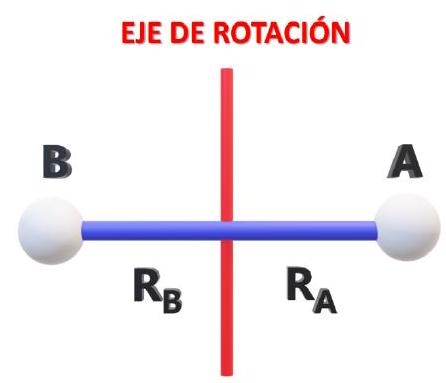
\includegraphics[scale = 0.30, center]{2025_04_01_ea720b93e8ebb5d0c6aeg-03}
    \caption{Sistema simple}
\end{figure}

Considerando un sistema compuesto por dos cuerpos A y B, los cuales están conectados por una barra de masa despreciable y giran alrededor de un eje que pasa por un punto de la barra, siendo este eje perpendicular a la misma con una velocidad angular $\vec{w}$, como se muestra en la figura 1; entonces, la energía cinética del sistema se expresa de la siguiente manera:


\begin{equation*}
E_{c}(\text { sistema })=\frac{1}{2} m_{A} v_{A}^{2}+\frac{1}{2} m_{B} v_{B}^{2} \tag{1}
\end{equation*}


Pero tenemos: $\left|\overrightarrow{v_{A}}\right|=v_{A}=|\vec{w}|\left|\overrightarrow{R_{A}}\right|=w R_{A}$ y $\left|\overrightarrow{v_{B}}\right|=v_{B}=|\vec{w}|\left|\overrightarrow{R_{B}}\right|=w R_{B}$. Reemplazando en 1:


\begin{equation*}
E_{c}(\text { sistema })=\frac{1}{2} m_{A} w^{2} R_{A}^{2}+\frac{1}{2} m_{B} w^{2} R_{B}^{2} \tag{2}
\end{equation*}


Vemos que, en el caso de la rotación, la energía cinética depende del eje elegido, por lo que debemos separar la energía cinética en el movimiento de traslación y rotación. Luego $E_{\text {rotacionalA }}=\frac{1}{2} m_{A} w^{2} R_{A}^{2}$ y $E_{\text {rotacional } B}=\frac{1}{2} m_{B} w^{2} R_{B}^{2}$

\subsection{Momento de inercia}
De 2 podemos factorizar $\frac{1}{2} w^{2}$.

$$
\begin{aligned}
E_{c}(\text { sistema }) & =\frac{1}{2} m_{A} w^{2} R_{A}^{2}+\frac{1}{2} m_{B} w^{2} R_{B}^{2} \\
& =\frac{1}{2}\left(m_{A} R_{A}^{2}+m_{B} R_{B}^{2}\right) w^{2} \\
& =\frac{1}{2} I w^{2}
\end{aligned}
$$

El momento de inercia del sistema en relación con el eje se define como $I = m_A R_A^2 + m_B R_B^2$, donde $R_A$ y $R_B$ representan las distancias de los cuerpos $A$ y $B$ al eje, respectivamente.  
Generalizando para un sistema discreto compuesto por $n$ partículas, la expresión correspondiente para el momento de inercia en torno a un eje es:


\begin{equation*}
\sum_{i=1}^{n} m_{i} R_{i}^{2} \tag{3}
\end{equation*}


Aquí, $m_i$ representa la masa de la i-ésima partícula, mientras que $R_i$ denota su distancia mínima al eje de rotación.  

Si en lugar de un sistema discreto consideramos un sistema de masa continua, la sumatoria se transforma en una integral, tomando un elemento diferencial de masa $(dm \rightarrow 0)$ cuya distancia mínima al eje de rotación es $r_i$.

\begin{equation*}
I=\lim _{d m_{i} \rightarrow 0} \sum r_{i}^{2} d m_{i} \tag{4}
\end{equation*}


Esto resulta ser la integral:


\begin{equation*}
I=\int r^{2} d m \tag{5}
\end{equation*}


Para resolver esta integral, hace falta saber como varía la masa respecto a la distancia mínima al eje de rotación.\\

Si el centro de masa del objeto es conocido y consideramos una lámina plana del mismo, es posible determinar el momento de inercia respecto a un eje paralelo a otro que atraviesa su centro de masa y que es perpendicular al plano de la lámina.
\begin{figure}[H]
    \centering
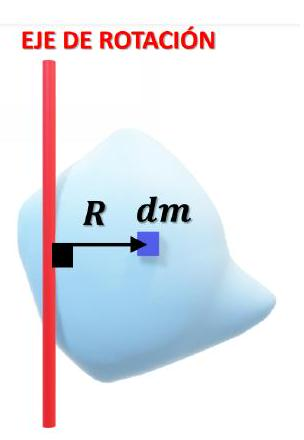
\includegraphics[scale = 0.30, center]{2025_04_01_ea720b93e8ebb5d0c6aeg-05}
\caption{Sistema de masas continuo}
\end{figure}


\begin{figure}[H]
    \centering
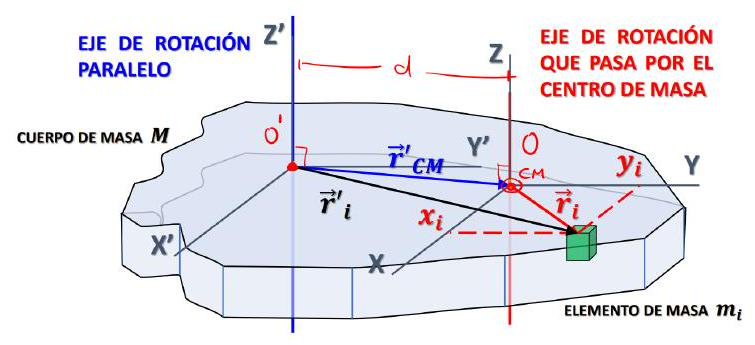
\includegraphics[scale = 0.30, center]{2025_04_01_ea720b93e8ebb5d0c6aeg-05(1)}
\caption{lámina plana del objeto. }
\end{figure}

Aquí, $\overrightarrow{r_{i}}$ representa la posición del elemento de masa $m_{i}$ en relación con el centro de masa (CM), mientras que ${\overrightarrow{r_{i}}}^{\prime}$ denota su posición con respecto al eje paralelo. Asimismo, $\overrightarrow{C M}^{\prime}$ es la posición del centro de masa en relación con dicho eje paralelo.
Luego, sabemos que : $\vec{r}_{i}^{\prime}=r_{C M}^{\prime}+\overrightarrow{r_{i}}, \sum_{i=1}^{n} m_{i} r_{i}^{\prime 2},{\overrightarrow{r_{i}}}^{\prime}={\overrightarrow{x_{i}}}^{\prime}+\vec{y}_{i}^{\prime}$ con $x_{i} \perp y_{i}$. Luego:

$$
\begin{aligned}
\sum_{i=1}^{n} m_{i} r_{i}^{\prime 2} & =\sum_{i=1}^{n} m_{i}\left({\overrightarrow{x_{i}}}^{\prime}+\vec{y}_{i}^{\prime}\right)^{2} \\
& =\sum_{i=1}^{n} m_{i}\left(x_{i}^{\prime 2}+y_{i}^{\prime 2}\right) \\
& =\sum_{i=1}^{n} m_{i}\left(x_{C M}^{\prime}+\overrightarrow{x_{i}}\right)^{2}+\sum_{i=1}^{n} m_{i}\left(y_{\overrightarrow{C M}}{ }^{\prime}+\vec{y}_{i}\right)^{2}
\end{aligned}
$$

Donde :\\
$\sum_{i=1}^{n} m_{i}\left(x_{C M}^{\prime}+\vec{x}_{i}\right)^{2}=\sum_{i=1}^{n} m_{i} x_{C M}^{\prime 2}+2 \sum_{i=1}^{n} m_{i}<x_{C M}^{\prime}, \vec{x}_{i}>+\sum_{i=1}^{n} m_{i} x_{i}^{2}$\\
$\sum_{i=1}^{n} m_{i}\left(\overrightarrow{C M}^{\prime}+\overrightarrow{y_{i}}\right)^{2}=\sum_{i=1}^{n} m_{i} y_{C M}^{\prime 2}+2 \sum_{i=1}^{n} m_{i}<y_{\text {CM }^{\prime}}, \overrightarrow{y_{i}}>+\sum_{i=1}^{n} m_{i} y_{i}^{2}$\\
Pero sabemos que $x_{\overrightarrow{C M}}{ }^{\prime}$ y $y_{\overrightarrow{C M}}{ }^{\prime}$ son constantes. entonces:

$$
\sum_{i=1}^{n} m_{i}<x_{\overrightarrow{C M}}{ }^{\prime}, \vec{x}_{i}>=<x_{C M}^{\prime}, \sum_{i=1}^{n} m_{i}{\overrightarrow{x_{i}}}^{\prime} y \sum_{i=1}^{n} m_{i}<y_{C M}{ }^{\prime}, \vec{y}_{i}>=<y_{C M}^{\prime}, \sum_{i=1}^{n} m_{i} \vec{y}_{i}>
$$

$$
\sum_{i=1}^{n} m_{i} \overrightarrow{x_{i}}=\sum_{i=1}^{n} m_{i}\left(\vec{x}_{i}^{\prime}-x_{C M}^{\prime}\right)=\overrightarrow{0}, \sum_{i=1}^{n} m_{i} \overrightarrow{y_{i}}=\sum_{i=1}^{n} m_{i}\left(\vec{y}_{i}^{\prime}-y_{C M}^{\prime}\right)=\overrightarrow{0}
$$

Entonces:

$$
\begin{aligned}
& \sum_{i=1}^{n} m_{i} r_{i}^{\prime 2}=\sum_{i=1}^{n} m_{i}\left(x_{C M}^{\prime 2}+y_{C M}^{\prime 2}\right)+\sum_{i=1}^{n} m_{i}\left(x_{i}^{2}+y_{i}^{2}\right) \\
& \text { Luego }: \\
& I_{\text {ejeparalelo }}=I_{C M}+M d^{2}
\end{aligned}
$$


Aquí, $d$ representa la distancia entre el eje paralelo y el eje que pasa por el centro de masa del sistema.  
Este razonamiento puede extenderse a todas las láminas que conforman el volumen del objeto, lo que sugiere que es válido para objetos en cualquier dimensión.  

Desde un punto de vista físico, el momento de inercia mide la resistencia de un cuerpo a rotar en torno a un eje dado.  
Es fundamental considerar la elección del eje de rotación, ya que el momento de inercia depende de este, pues modificar el eje implica alterar las distancias de los elementos de masa con respecto a él.
\subsection{Dinámica de cuerpo rígido}
Definimos al torque de una fuerza como una cantidad asociada a la capacidad de la fuerza, de alterar el estado de rotación de un cuerpo rígido.\\

\begin{figure}[H]
    \centering
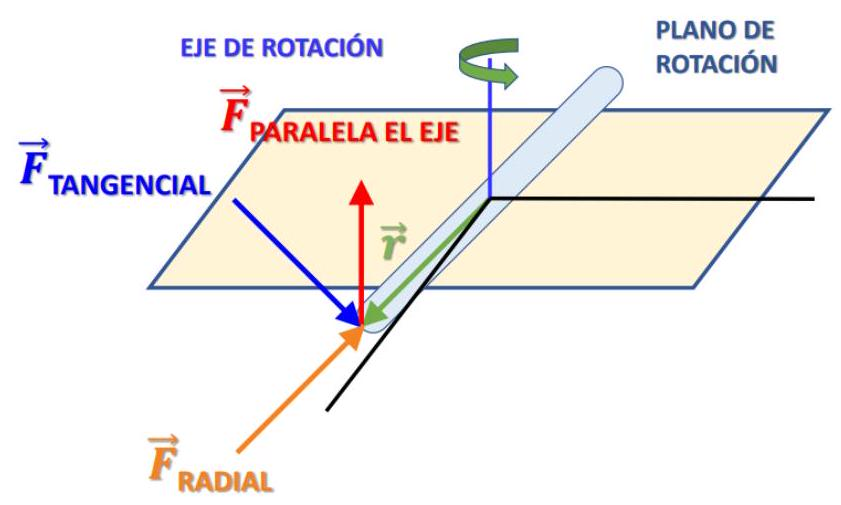
\includegraphics[scale = 0.30, center]{2025_04_01_ea720b93e8ebb5d0c6aeg-06}
\caption{Representación del torque de una fuerza }
\end{figure}


Observamos que únicamente la fuerza tangencial, $F_{\text{tangencial}}$, es capaz de modificar el estado de rotación en relación con el punto de aplicación y el eje de rotación.  
Esto se debe a que solo esta fuerza genera un cambio en la velocidad tangencial, y dado que $|\vec{v}| = |\vec{\omega}| \cdot |\vec{r}|$, se concluye que $\vec{\omega}$ aumenta.  

Además, el sentido de giro está determinado por la dirección del vector $\vec{r} \times \vec{F}$.  
De este modo, podemos establecer la siguiente expresión para el torque debido a la fuerza aplicada:  
\[
{\overrightarrow{\tau_{\text{eje}}}}^{F} = \vec{r} \times \vec{F}
\]  

Si la separación respecto al eje de rotación es suficientemente amplia para tratar al cuerpo rígido como una partícula, se introduce una nueva magnitud vectorial conocida como momento angular, definida por la expresión:
\[
\vec{L} = \vec{r} \times \vec{p}
\]
donde
\begin{figure}[H]
    \centering
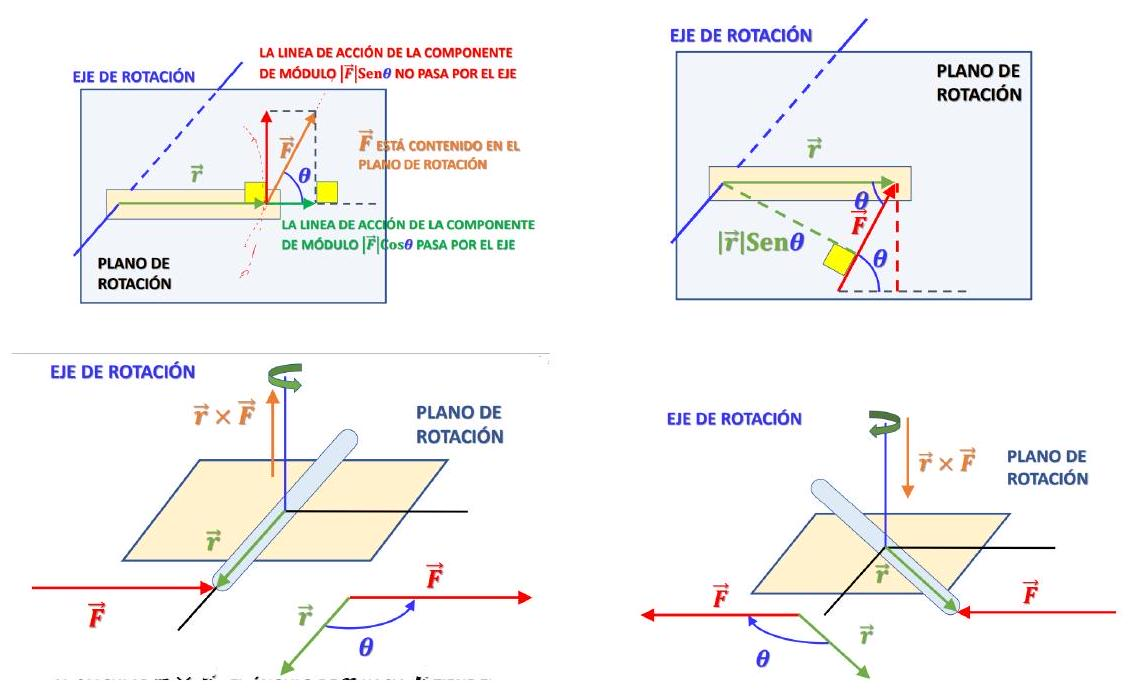
\includegraphics[scale = 0.30, center]{2025_04_01_ea720b93e8ebb5d0c6aeg-07(1)}
\caption{Representación de $\vec{r} \times \vec{F}$ y su relación con el torque}
\end{figure}

$p$ es la cantidad de movimiento lineal y r es la posición del cuerpo rígido respecto al eje de giro).\\

\begin{figure}[H]
    \centering
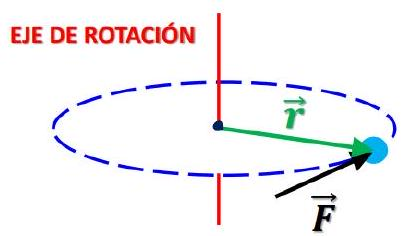
\includegraphics[scale = 0.30, center]{2025_04_01_ea720b93e8ebb5d0c6aeg-07}
\caption{Se desprecian las dimensiones del cuerpo rígido }
\end{figure}

Si derivamos $\vec{L}$ respecto al tiempo, tenemos:

$$
\begin{aligned}
\frac{d \vec{L}}{d t} & =\frac{d(\vec{r} \times \vec{p})}{d t} \\
& =\vec{r} \times \frac{d \vec{p}}{d t}+\frac{d \vec{r}}{d t} \times \vec{p} \\
& =\vec{r} \times \vec{F}+m \vec{v} \times \vec{v} \\
& =\vec{r} \times \vec{F} \\
& =\overrightarrow{t_{e j e}}
\end{aligned}
$$


Luego, si seleccionamos el eje adecuado de modo que $\vec{L} \| \vec{w}$ (y se cumple que: $\vec{r} \perp \vec{w}$), obtenemos:
\[
\vec{L} = m \vec{r} \times (\vec{w} \times \vec{r}) = m (\langle \vec{r}, \vec{r} \rangle \vec{w} - \langle \vec{w}, \vec{r} \rangle \vec{r}) = m r^{2} \vec{w} = I \vec{w}
\]
donde $I$ es el momento de inercia del cuerpo rígido respecto al eje. Luego, al derivar, obtenemos:
\[
\overrightarrow{\tau_{e j e}^{F}} = I \vec{\alpha}
\]
donde $\vec{\alpha}$ es la aceleración angular.
\subsection{ Movimiento de rodadura}

Un caso particular de la combinación del movimiento de traslación y rotación de un cuerpo rígido (en este caso, una rueda simétrica) es el movimiento de rodadura pura (rueda sin deslizamiento). Físicamente, el no deslizamiento implica que el punto de contacto entre
\begin{figure}[H]
    \centering
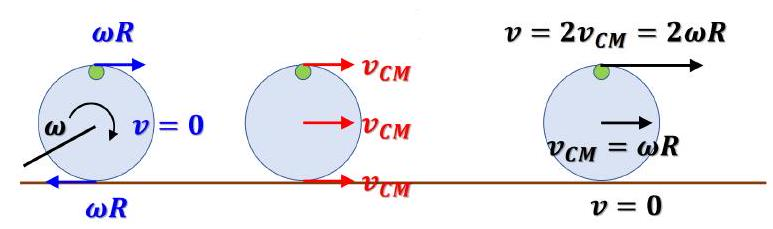
\includegraphics[scale = 0.30, center]{2025_04_01_ea720b93e8ebb5d0c6aeg-08(1)}
\caption{Rotación+Traslación sin resbalar}
\end{figure}

La rueda y la superficie no experimentan desplazamiento ni velocidad en el punto de contacto, como resultado de las condiciones iniciales: $v_{C M} = w R$; este punto se denomina centro instantáneo de rotación (CIR), ya que la rueda parece girar alrededor de un eje instantáneo perpendicular al plano de la rueda que pasa por el punto de contacto. De esto, concluimos que la rueda únicamente realiza rotación respecto al CIR, por lo que, si existen pérdidas, estas se deben a la rotación y no a la traslación. Sin embargo, podemos reformular la expresión en términos de las características del centro de masa (su velocidad y el momento de inercia respecto a un eje que pasa por el centro de masa y es perpendicular al plano de la rueda).
$$
\begin{aligned}
E_{\text {rotacional }} & =\frac{1}{2} I_{C I R} w^{2} \\
& =\frac{1}{2}\left(I_{C M}+m R^{2}\right) w^{2} \\
& =\frac{1}{2} I_{C M} w^{2}+\frac{1}{2} m(w R)^{2} \\
& =\frac{1}{2} I_{C M} w^{2}+\frac{1}{2} m v_{C M}^{2} \\
& =E_{\text {rotacional } / C M}+E_{\text {traslacional } / C M}
\end{aligned}
$$

Donde $m$ es la masa de la rueda.\\
En el caso ideal, la rueda y la superficie no se deforman por acción de las fuerzas. Como\\

\begin{figure}[H]
    \centering
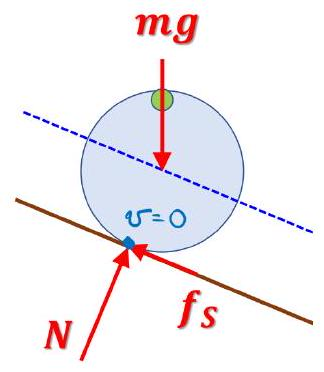
\includegraphics[scale = 0.30, center]{2025_04_01_ea720b93e8ebb5d0c6aeg-08}
\caption{DCL de la rueda en un plano inclinado.}
\end{figure}

El punto de contacto no experimenta desplazamiento, $W_{f s} = W_{F N C} = 0$, y por lo tanto, se conserva la energía mecánica.\\
En un escenario real, se toman en cuenta las deformaciones de la rueda y la superficie, y además, se observa que la rueda desliza debido a las deformaciones. Este fenómeno se conoce como fricción por rodadura.\\
\begin{figure}[H]
    \centering
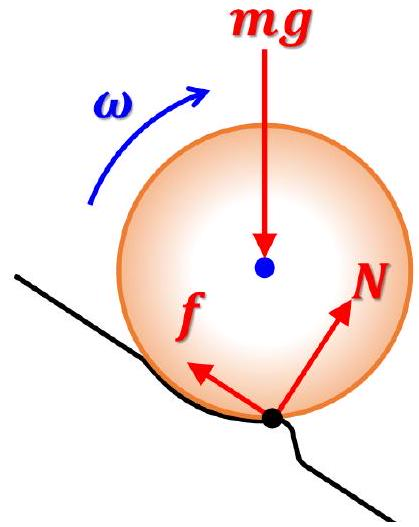
\includegraphics[scale = 0.30, center]{2025_04_01_ea720b93e8ebb5d0c6aeg-09}
\caption{Se aprecian deformaciones}
\end{figure}


Esto genera una pérdida de energía mecánica; sin embargo, es frecuente ignorar este efecto en experimentos reales, dado que la rueda y la superficie son lo suficientemente rígidas como para no notar efectos significativos debido a la fricción por rodadura. Por lo tanto, se considera que la energía mecánica se conserva también en estos casos.

\subsection{Aplicaciones en el experimento}

Contamos con una rueda de Maxwell proporcionada en el laboratorio, la cual posee un eje perpendicular al plano de la rueda que pasa por su centro de gravedad. El eje es un cilindro concéntrico con la rueda, cuyo radio $\mathrm{r} < \mathrm{R}$ (siendo $\mathrm{R}$ el radio de la rueda), similar a lo mostrado en la figura (a). En la figura 10b, se encuentran marcados los puntos $A_{0}, A_{1}, A_{2}$,
\begin{figure}[H]
    \centering
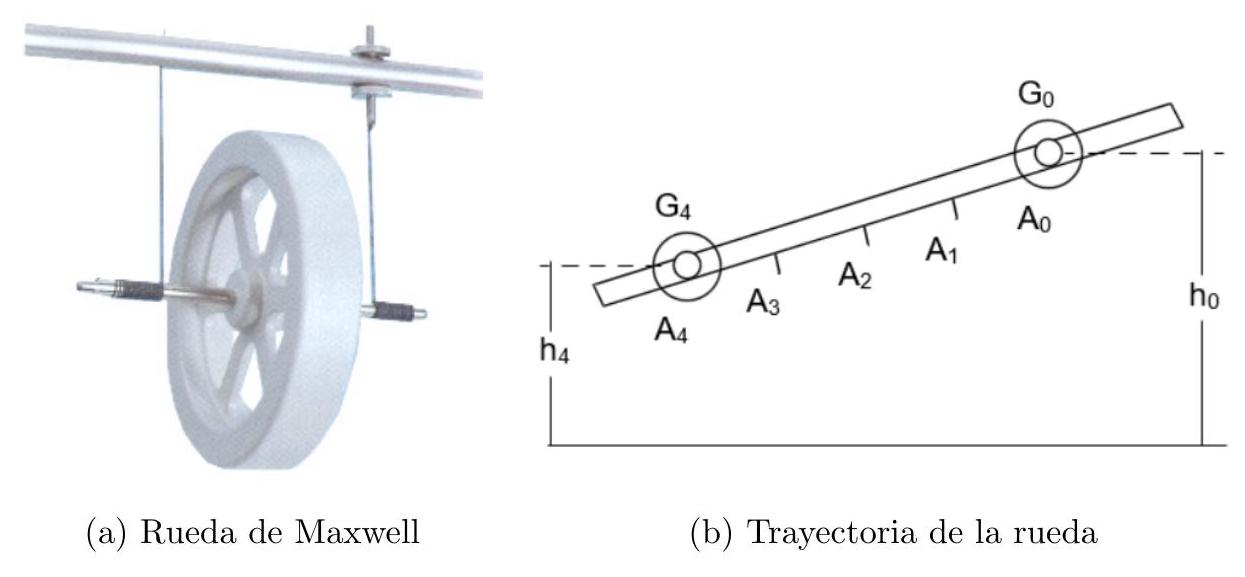
\includegraphics[scale = 0.30, center]{2025_04_01_ea720b93e8ebb5d0c6aeg-09(1)}
\end{figure}

$A_{3}$ y $A_{4}$ están separados por 10 cm; también contamos con $G_{0}$ y $G_{4}$, que representan las posiciones del centro de gravedad de la rueda, en el punto más alto y más bajo de su trayectoria, respectivamente. Debido a todo lo mencionado anteriormente, se desprecia la fricción por rodadura, y por lo tanto, se conserva la energía mecánica. Por lo que:

\begin{align*}
E_{M(4)} & =m g h_{4}+\frac{1}{2} I_{G} w_{G_{4}}^{2}+\frac{1}{2} m v_{G_{4}}^{2}  \tag{6}\\
& =m g h_{4}+\frac{1}{2} I_{G} \frac{v_{G_{4}}^{2}}{r^{2}}+\frac{1}{2} m v_{G_{4}}^{2}  \tag{7}\\
& =E_{M(0)}  \tag{8}\\
& =m g h_{0}+\frac{1}{2} I_{G} \frac{v_{G_{0}}^{2}}{r^{2}}+\frac{1}{2} m v_{G_{0}}^{2}  \tag{9}\\
m g h_{0}\left(v_{G_{0}}=0\right) & =m g h_{4}+\frac{1}{2} I_{G} \frac{v_{G_{4}}^{2}}{r^{2}}+\frac{1}{2} m v_{G_{4}}^{2} \tag{10}
\end{align*}

Posteriormente, $x = \frac{1}{2} a t^{2}$ en relación con el centro de masa, dado que la posición inicial es $x = 0$ y se observa un MRUV en la rueda, generado por una aceleración constante debido al peso, la fricción estática y la fuerza normal. Sabemos que $v_{G} = a t$ cuando $v_{0} = 0$, por lo que $v_{G} = \frac{2 x}{t}$. Con estos datos, podemos realizar el experimento y comprobar los resultados, midiendo únicamente la velocidad, el radio del eje de rotación, el desplazamiento y el tiempo transcurrido.
\section{Equipo utilizado y diagrama de flujo del experimento}
\subsection{Equipo utilizado}
\begin{itemize}
  \item Un par de rieles paralelos (como plano inclinado)
\begin{figure}[H]
    \centering
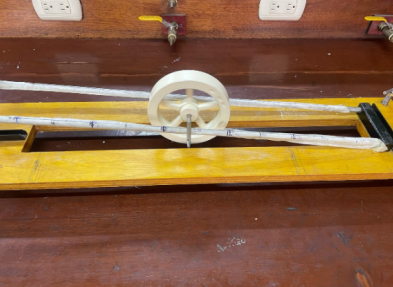
\includegraphics[scale = 0.40, center]{rieles}
\end{figure}
          
  \item Una rueda de Maxwell
\begin{figure}[H]
    \centering
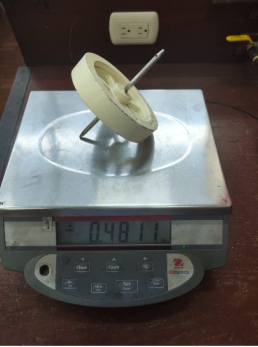
\includegraphics[scale = 0.40, center]{rueda}
\end{figure}
  \item Un cronómetro digital
\begin{figure}[H]
    \centering
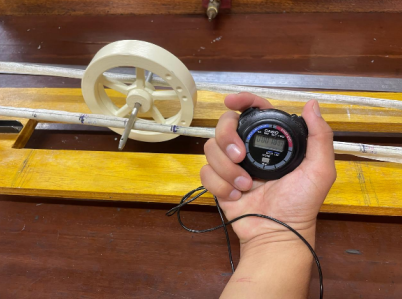
\includegraphics[scale = 0.40, center]{cronometro}
\end{figure}
  \item Un pie de rey
\begin{figure}[H]
    \centering
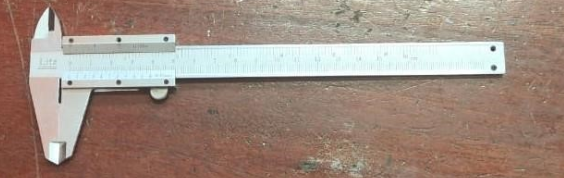
\includegraphics[scale = 0.40, center]{vernier}
\end{figure}
  \item Una regla milimetrada
\begin{figure}[H]
    \centering
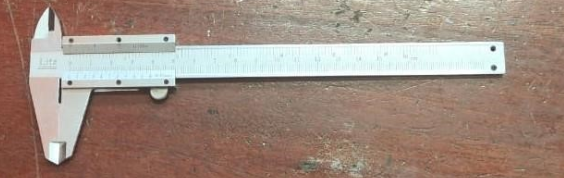
\includegraphics[scale = 0.40, center]{vernier}
\end{figure}
  \item Una balanza
\begin{figure}[H]
    \centering
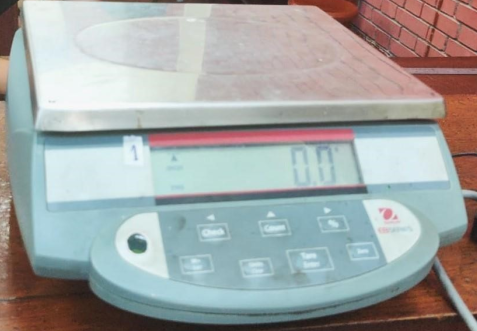
\includegraphics[scale = 0.40, center]{balanza}
\end{figure}
  \item Un nivelador
\begin{figure}[H]
    \centering
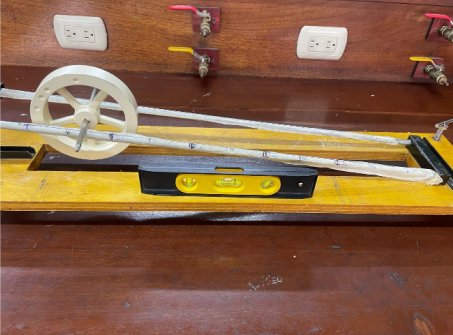
\includegraphics[scale = 0.40, center]{nivel}
\end{figure}
\end{itemize}

\subsection{Diagrama de Flujo}
\begin{figure}[H]
    \centering
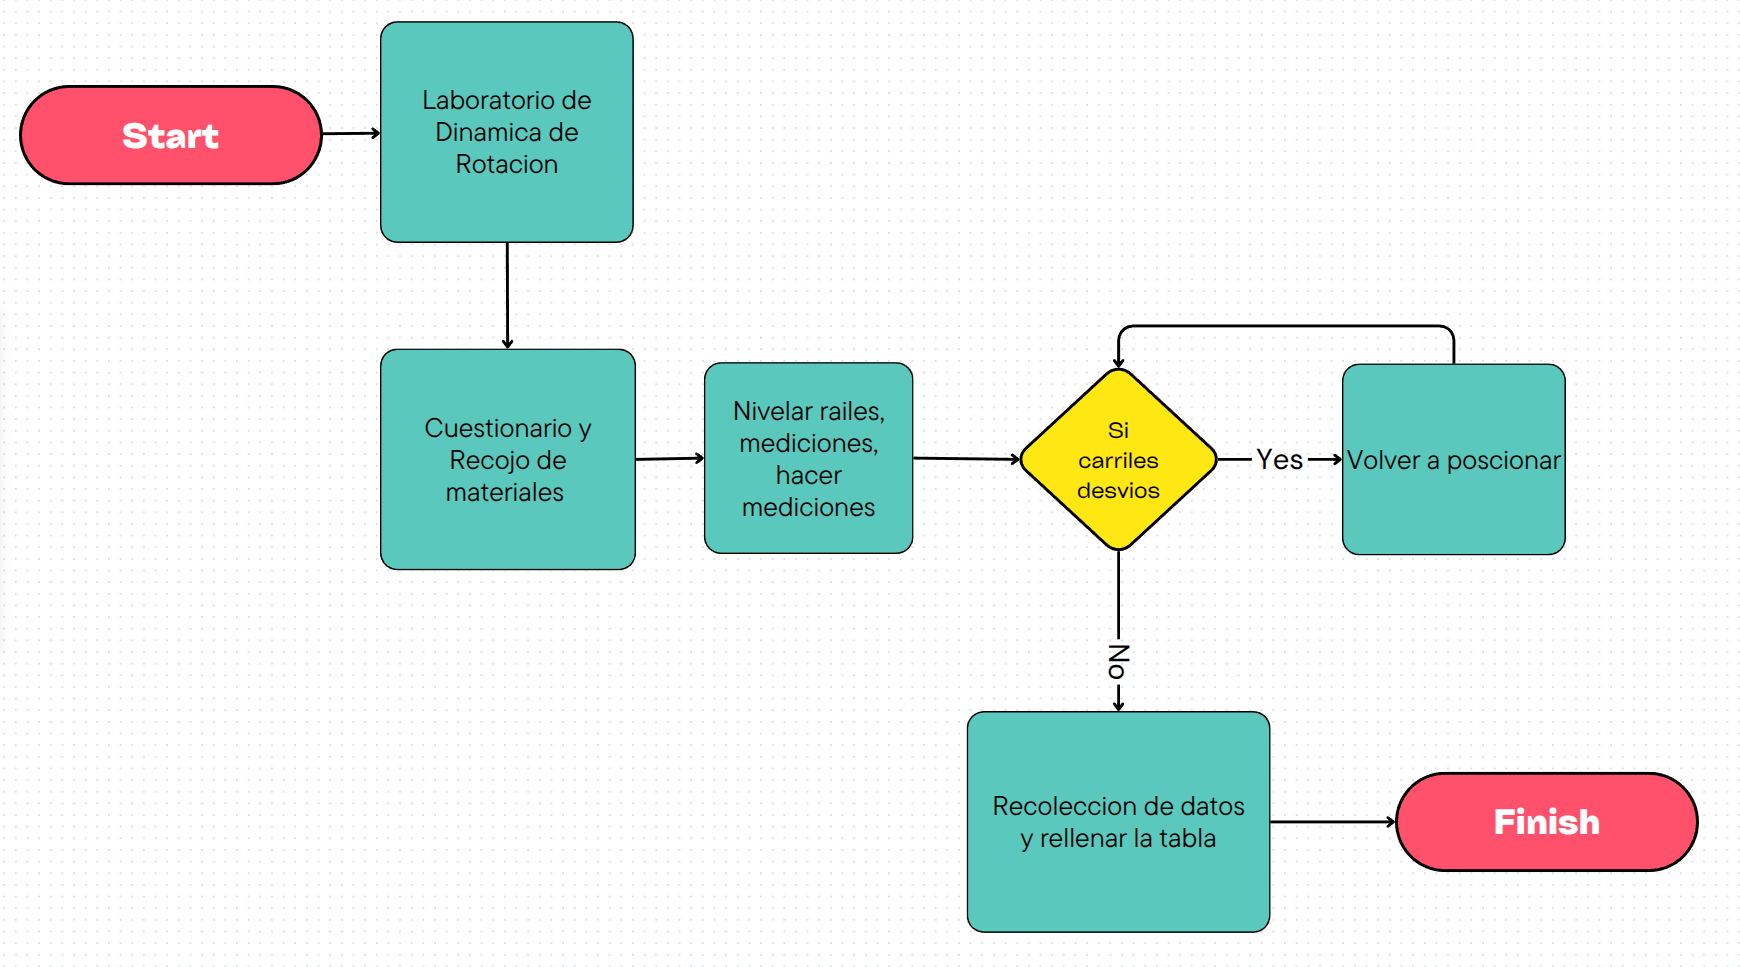
\includegraphics[scale = 0.30, center]{Diagrama}
\caption{Diagrama de Flujo}
\end{figure}
\end{itemize}

\section{Procedimiento Experimental}
\begin{itemize}
\end{itemize}
\section{C\'{a}lculos y resultados}
\section{Cuestionario}
\section{Conclusiones}
\section{Anexo}



\end{document}

